\chapter{Patterns et descriptions techniques}

\section{Librairies externes utilisées}

Afin de pouvoir implémenter une partie de nos fonctionnalités principales et d'optimiser l'expérience utilisateur de l'application, nous avons eu à faire recours à plusieurs bibliothèques externes. Pour cela, il a avant tout fallu se documenter à propos des bibliothèques existantes et avoir des avis sur celles-ci afin de s'assurer qu'elles soient bien stables, à jour, et qu'elles fournissent tous les services qui nous sont nécessaires.\\

L'application utilise cinq bibliothèques externes: \\

\begin{itemize}
\renewcommand{\labelitemi}{$\bullet$}
\item \textbf{UnboundID LDAP SDK}: indispensable pour la connexion aux serveurs utilisant le protocole LDAP étant donné que la SDK de Java ne fournit aucun outil équivalent. On avait également encore le choix avec \textit{JNDI LDAP} et \textit{Spring LDAP} qui sont deux bibliothèques LDAP connues mais beaucoup plus complexes à utiliser et obsolètes. \\
\item \textbf{Jsoup}: la bibliothèque de référence pour l'analyse textuelle de textes HTML. Elle sert a parser les événements ainsi que l'annuaire du LaBRI. \\
\item \textbf{Google Play Services lib}: librairie nécessaire pour utiliser les services de Google Maps et donc implémenter les services affectant le plan du campus. \\
\item \textbf{Sliding menu lib}: sert à améliorer l'esthétique et l'expérience utilisateur au sein du service qui affiche les événements. Permet de rajouter une barre latérale qui sert à basculer entre les différentes catégories d'événements à tout moment en faisant un simple geste de glissement avec le doigt. \\
\item \textbf{Robotium}: bibliothèque spécifique à la plateforme Android qui nous a été utile durant la phase finale du projet afin d'effectuer des tests en boîte noire pour notre interface graphique. 
\end{itemize}

\section{Extraction des dates}
L’extraction des dates se fait a l’aide d’expressions régulières que l’on applique au contenu des événements. Nous détectons les dates “standalone” pour marquer le début des événements, mais aussi les intervalles de dates afin de pouvoir préciser une durée d’événement lorsque l’utilisateur se décide à ajouter l’événement au calendrier de son téléphone.

\section{Recyclage de vues dans ListView}
Android fournit des outils pour la gestion des listes graphiques, notamment ListView couplée avec l’interface ListAdapter.\\
ListView est conçue pour être extensible et performante, ce qui signifie:

\begin{enumerate}
\item ListView va essayer d’effectuer des inflations de vues aussi peu que possible.
\item ListView ne va dessiner et disposer ses fils que quand ils sont visibles sur l’écran (ou sur le point de l'être).
\end{enumerate}

Le point 1 se justifie par le fait que les opérations d’inflation de layout sont coûteuses (de l’ordre de 1kB de RAM par vue). Ce problème est résolu par le recyclage des vues non visibles, qu’on appelle \emph{ScrapView}. Cela signifie qu’on peut utiliser des vues recyclées et les mettre à jour, au lieu de faire des inflations de vues pour chaque rangée.

Afin d’implémenter le point 2, ListView utilise un recycleur de vues qui déplacera les vues actives dans une pool recyclable quand elles sortent de l’écran. Ainsi, //TODO

\begin{figure}[h]
  \center
  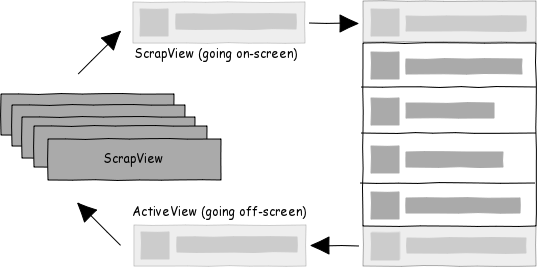
\includegraphics[width=0.92\textwidth]{resources/listview_recycling.png}
\end{figure}

A chaque fois que ListView a besoin d’afficher une nouvelle ligne sur l’écran, elle appelle la méthode \emph{getView()} depuis son adapter.

\begin{adjustbox}{minipage=1.12\textwidth,margin=0pt \smallskipamount,center}
\begin{lstlisting}[style=Java, label=listview1]
public View getView(int position, View convertView, ViewGroup parent)
\end{lstlisting}
\end{adjustbox}

L’argument \emph{convertView} est essentiellement une vue recyclée (\emph{ScrapView}), comme indiqué précédemment. Quand il aura une valeur non nulle, il faudra donc en profiter pour simplement mettre à jour les données au lieu de faire une nouvelle inflation de layout.

\begin{adjustbox}{minipage=1.14\textwidth,margin=0pt \smallskipamount,center}
\begin{lstlisting}[style=Java, label=listview2]
public View getView(int position, View convertView, ViewGroup parent){ 
	View item = mInflater.inflate(R.layout.list_item_icon_text, null);
	((TextView) item.findViewById(R.id.text)).setText(DATA[position]); 
	((ImageView) item.findViewById(R.id.icon)).setImageBitmap(mIcon);
	return item; 
}
\end{lstlisting}
\end{adjustbox}
